\documentclass[utf8]{article}

\usepackage[utf8]{inputenc}

\usepackage[parfill]{parskip}

\usepackage{amsmath}
\usepackage{mathtools}
\usepackage{nccmath}
\usepackage{amssymb}
\usepackage{amsfonts}
\usepackage{graphicx}
\usepackage{caption}
\usepackage{subcaption}
\usepackage{float}
\usepackage{listingsutf8}
\usepackage{hyperref}
\usepackage[dvipsnames]{xcolor}
\usepackage{comment}

\usepackage{fullpage}

%------------------------------------------------------

\usepackage{listings}
\usepackage{adjustbox}

\definecolor{color0}{RGB}{147, 147, 147}
\definecolor{color1}{RGB}{186, 033, 033}
\definecolor{color2}{RGB}{000, 128, 000}
\definecolor{color3}{RGB}{064, 128, 128}
\definecolor{color4}{RGB}{170, 034, 255}

\lstdefinelanguage{clips}{
  mathescape = true,
  sensitive        = true,
  morecomment      = [l]{;},
  showstringspaces = false,
  morestring       = [b]",
}

% egreg's modulo macro (see https://tex.stackexchange.com/a/34449/21891)
\def\truncdiv#1#2{((#1-(#2-1)/2)/#2)}
\def\moduloop#1#2{(#1-\truncdiv{#1}{#2}*#2)}
\def\modulo#1#2{\number\numexpr\moduloop{#1}{#2}\relax}


\makeatletter

% a TeX counter to keep track of the nesting level
\newcount\netParensCount@clisp

% Modify how ( and ) get typeset depending on the value of the counter
% (Based on Ulrike Fischer's approach to modifying characters in listings;
% see https://tex.stackexchange.com/a/231927/21891)
\lst@CCPutMacro
\lst@ProcessOther{`(}{{%
  \ifnum\lst@mode=\lst@Pmode\relax%
    \rainbow@clisp{(}%
    \global\advance\netParensCount@clisp by \@ne%
  \else
    (%
  \fi
}}%
\lst@ProcessOther{`)}{{%
  \ifnum\lst@mode=\lst@Pmode\relax%
    \global\advance\netParensCount@clisp by \m@ne%
    \rainbow@clisp{)}%
  \else
    )%
  \fi
}}%
\@empty\z@\@empty

% Color its argument based on the value of the \netParensCount@clisp counter
% (modulo 5)
\newcommand\rainbow@clisp[1]{%
  \ifcase\modulo\netParensCount@clisp 5\relax%
    \textcolor{color0}{#1}%
  \or
    \textcolor{color1}{#1}%
  \or
    \textcolor{color2}{#1}%
  \or
    \textcolor{color3}{#1}%
  \else
    \textcolor{color4}{#1}%
  \fi
}

\lst@AddToHook{PreInit}{%
  \global\netParensCount@clisp 0\relax%
}

\makeatother

\lstnewenvironment{clips-code}
  {\lstset{language=clips}}
  {}

\setcounter{tocdepth}{6}
\setcounter{secnumdepth}{6}

% -----------------------------------------------------


\title{INFO-F-305 - Modélisation et Simulation
\\Projet Octave
\\Wall-e}
\author{Becker Robin-Gilles - Bourgeois Noé}
\date{December 2022}

\begin{document}
\maketitle
\tableofcontents

\newpage

% -----------------------------------------------------

\section{Introduction}
Ce projet consiste à modéliser une relation amoureuse utilisant les systèmes dynamiques. Nous allons modéliser l'évolution de leurs sentiments ainsi qu'étudier les types de portraits de phase des différents systèmes d'après leurs valeurs a et b.

\section{Systèmes}

Pour modéliser l'évolution des sentiments de Wall-E, en bleu, et d'Eve, en orange, nous avons fixé a et b respectivement à -0.15 et 0.9.
\\
Pour dessiner les portraits de phase, nous avons fixé les conditions initiales à -1 et 1.
\\
Tout a été réalisé sur un intervalle de temps de 0 à 10.


\subsection{Les sentiments d’EVE ne dépendent pas de WALL-E}

\begin{equation}
\centering
\left\{\begin{split}
\dot{w}(t) &= aw(t) + be(t)\\
\dot{e}(t) &= 0 \\
\end{split}\right.
 \end{equation}

\begin{equation}
\centering
A = \left[
\begin{array}{cc}
a & b\\
0 & 0
\end{array}
\right]
 \end{equation}


\begin{figure}[!htb]
\centering
\begin{subfigure}{.3\textwidth}
  \centering
  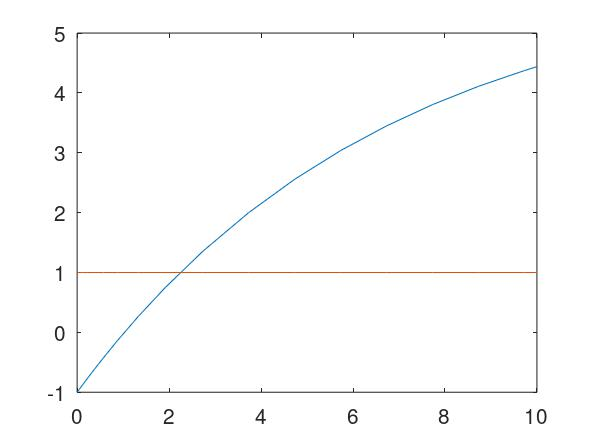
\includegraphics[width=\linewidth]{évol/E1-1_1.jpg}
  \caption{y0 = [-1,1]}
  \label{fig:sub1}
\end{subfigure}%
\begin{subfigure}{.3\textwidth}
  \centering
  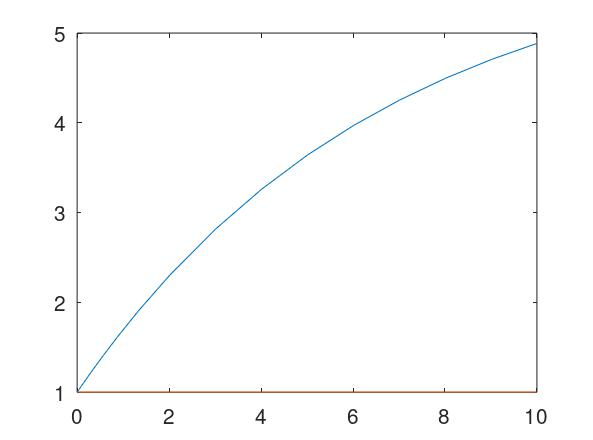
\includegraphics[width=\linewidth]{évol/E11_1.jpg}
  \caption{y0 = [1,1]}
  \label{fig:sub2}
  \end{subfigure}
  \begin{subfigure}{.3\textwidth}
  \centering
  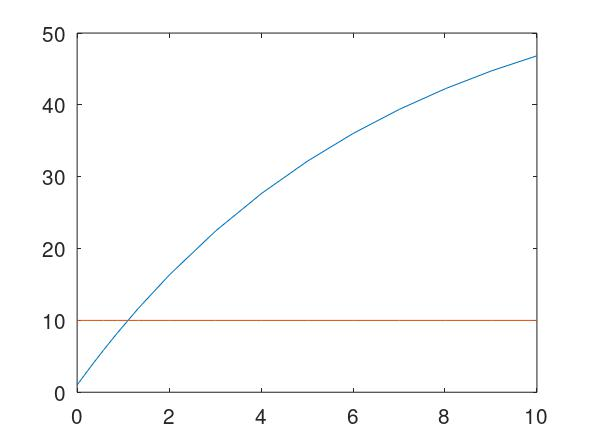
\includegraphics[width=\linewidth]{évol/E11_10.jpg}
  \caption{y0 = [1,10]}
%  \label{fig:sub1}
  \end{subfigure}%
  \begin{subfigure}{.3\textwidth}
  \centering
  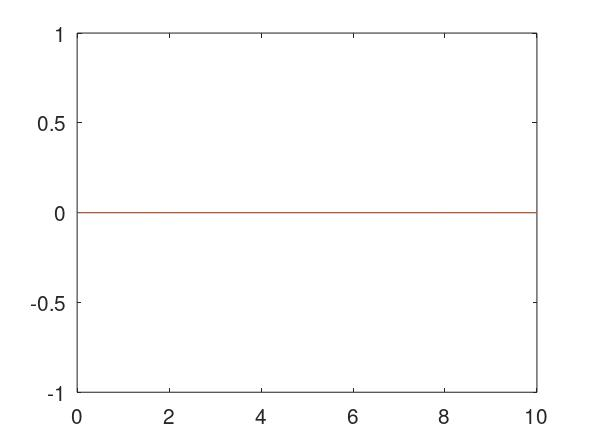
\includegraphics[width=\linewidth]{évol/E10_0.jpg}
  \caption{y0 = [0,0]}
%  \label{fig:sub2}
  \end{subfigure}
  \begin{subfigure}{.3\textwidth}
  \centering
  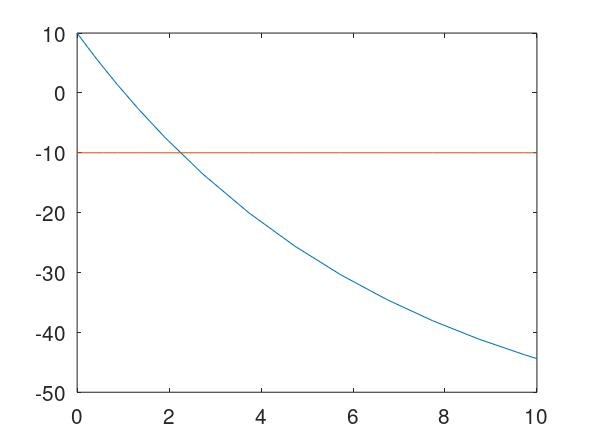
\includegraphics[width=\linewidth]{évol/E110_-10.jpg}
  \caption{y0 = [10,-10]}
%  \label{fig:sub2}
  \end{subfigure}
\caption{Evolutions du système 1 pour les conditions initiales y0}
%\label{fig:test}
\end{figure}

\subsubsection{Typologie}

Si a $<$ 0, cela donne un noeud stable dégénéré. Ici, a = -0.15 et b = 0.9.
\\
Si a $>$ 0, cela donne un noeud instable dégénéré. Ici, a = -0.15 et b = 0.9.
\\
Si a = 0, cela donne un noeud singulier. Ici a = 0 et b = 1.

\begin{figure}[!htb]
\centering
\begin{subfigure}{.5\textwidth}
  \centering
  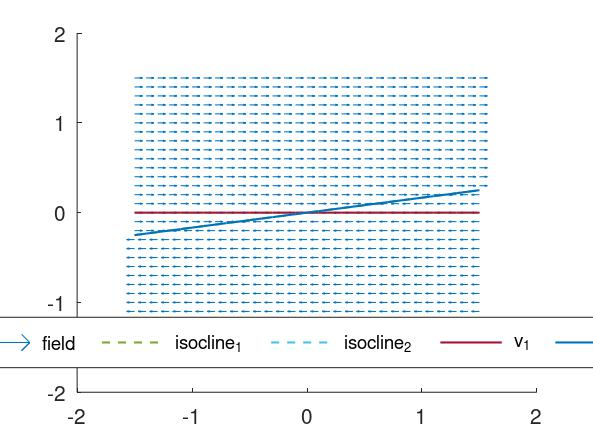
\includegraphics[width=\linewidth]{Phases/P1-015_09.jpg}
  \caption{a = -0.15 et b = 0.9}
  \label{fig:sub1}
\end{subfigure}%
\begin{subfigure}{.5\textwidth}
  \centering
  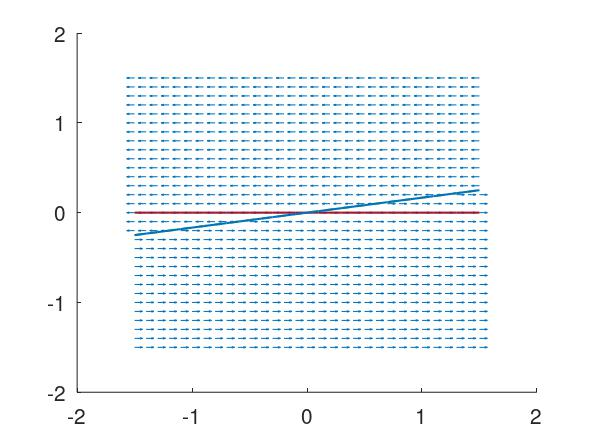
\includegraphics[width=\linewidth]{Phases/P1015_-09.jpg}
  \caption{a = 0.15 et b = -0.9}
  \label{fig:sub2}
  \end{subfigure}
  \begin{subfigure}{.5\textwidth}
  \centering
  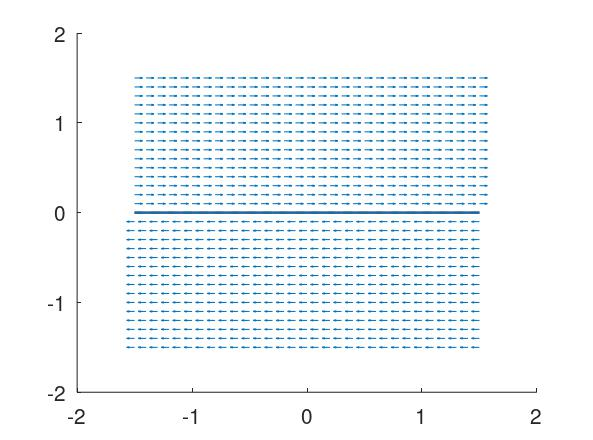
\includegraphics[width=\linewidth]{Phases/P10_1.jpg}
  \caption{a = 0 et b = 1}
%  \label{fig:sub1}
  \end{subfigure}%
\caption{Portraits de phase du système 1}
%\label{fig:test}
\end{figure}

\newpage

\subsection{Les deux robots ont la même dynamique}

\begin{equation}
\centering
\left\{\begin{split}
\dot{w}(t) &= aw(t) + be(t)\\
\dot{e}(t) &= bw(t) + ae(t) \\
\end{split}\right.
 \end{equation}

On peut en déduire la matrice à coefficients A telle que X˙ (t) = Ax :

% coefficients matrix A
\begin{equation}
\centering
A = \left[
\begin{array}{cc}
a & b\\
b & a
\end{array}
\right]
 \end{equation}

De là, nous pouvons décider d’utliser le diagramme de Pointcarré
ou la méthode des valeurs propres
pour définir le type de système (selle, nœud stable, ….)
Dans cet exemple, nous allons utiliser
les valeurs propres.
On calcule les valeurs propres en posant l’équation caractéristique :

\begin{equation}
\centering
\det(A − λI) = 0
 \end{equation}

On résoud et on obtient les valeurs propres :

\begin{equation}
\centering
\lambda_1,2 = 2a \pm \sqrt{4b^2} = {a - b, a + b}
 \end{equation}

On distingue les différents cas possibles :
1. Selle : pour que le système soit une selle, il faut
λ1,2 ̸= 0
et
signe(λ1) ̸= signe(λ2). On a


\begin{figure}[!htb]
\centering
\begin{subfigure}{.3\textwidth}
  \centering
  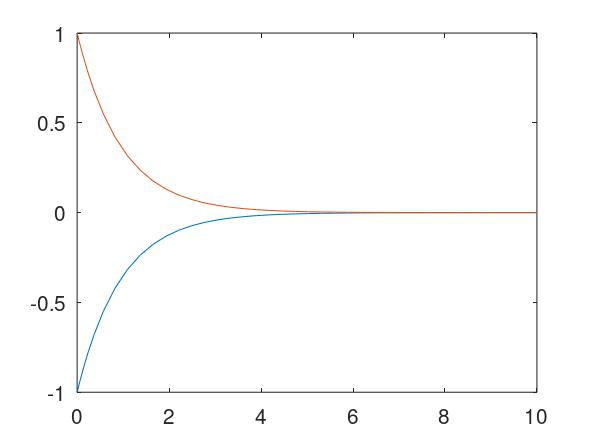
\includegraphics[width=\linewidth]{évol/E2-1_1.jpg}
  \caption{y0 = [-1,1]}
  \label{fig:sub1}
\end{subfigure}%
\begin{subfigure}{.3\textwidth}
  \centering
  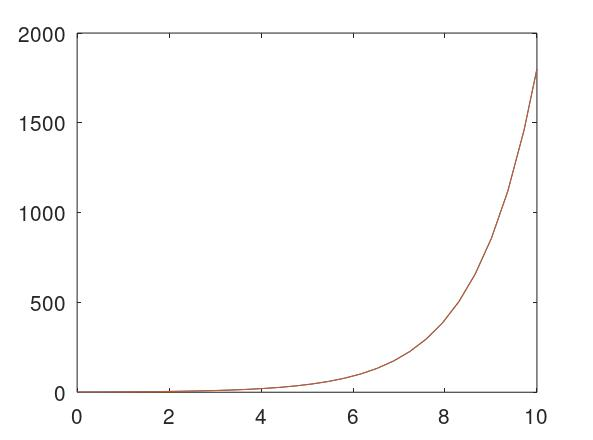
\includegraphics[width=\linewidth]{évol/E21_1.jpg}
  \caption{y0 = [1,1]}
  \label{fig:sub2}
  \end{subfigure}
  \begin{subfigure}{.3\textwidth}
  \centering
  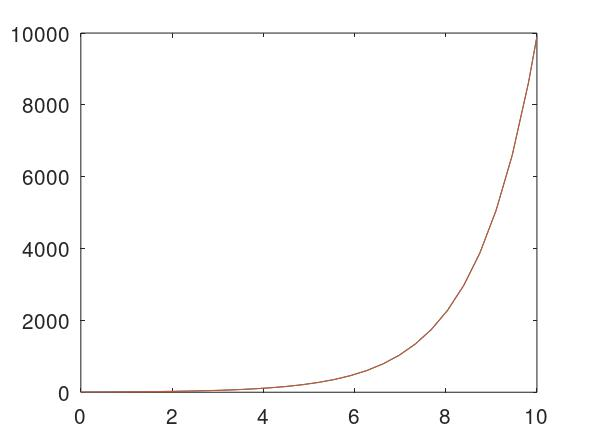
\includegraphics[width=\linewidth]{évol/E21_10.jpg}
  \caption{y0 = [1,10]}
%  \label{fig:sub1}
  \end{subfigure}%
  \begin{subfigure}{.3\textwidth}
  \centering
  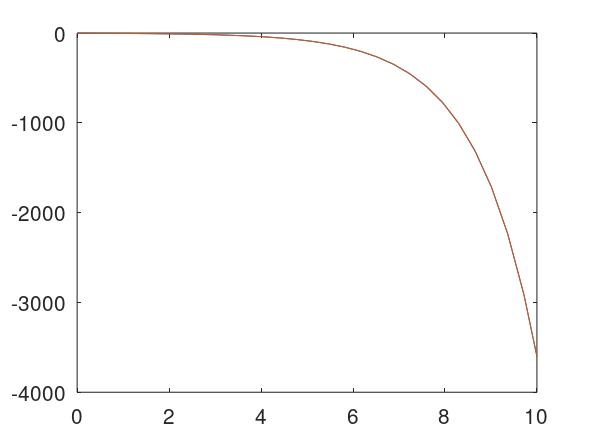
\includegraphics[width=\linewidth]{évol/E2-2_-2.jpg}
  \caption{y0 = [-2,-2]}
%  \label{fig:sub2}
  \end{subfigure}
  \begin{subfigure}{.3\textwidth}
  \centering
  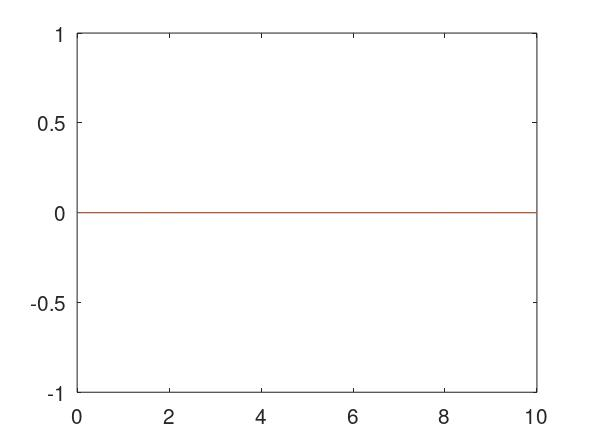
\includegraphics[width=\linewidth]{évol/E20_0.jpg}
  \caption{y0 = [0,0]}
%  \label{fig:sub2}
  \end{subfigure}
\caption{Evolutions du système 2 pour les conditions initiales y0}
%\label{fig:test}
\end{figure}

\subsubsection{Typologie}

Si a $< -|b|$ , cela donne un noeud stable. Ici, 0.15 $<$ -(-0.9)
\\
Si a $ > -|b|$, cela donne un noeud instable. Ici, a = 1 et b = 0.1.
\\
Si -b $<$ a $<$ b, cela donne une selle. Ici, -(0.9) $<$ -0.15 $<$ 0.9
\\
Si a = b $<$ 0, cela donne une ligne de points d’équilibre stable. Ici, a et b = -0.1.
\\
Si a = b $>$ 0, cela donne une ligne de points d’équilibre instable. Ici, a et b = 0.1.

\begin{figure}[!htb]
\centering
\begin{subfigure}{.5\textwidth}
  \centering
  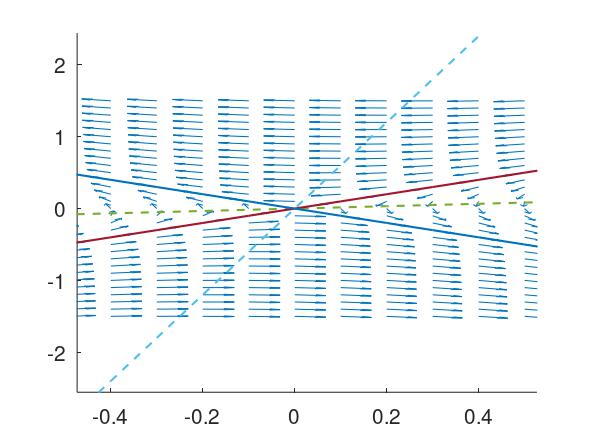
\includegraphics[width=\linewidth]{Phases/P2015_-09.jpg}
  \caption{a = 0.15 et b = -0.9}
  \label{fig:sub1}
\end{subfigure}%
\begin{subfigure}{.5\textwidth}
  \centering
  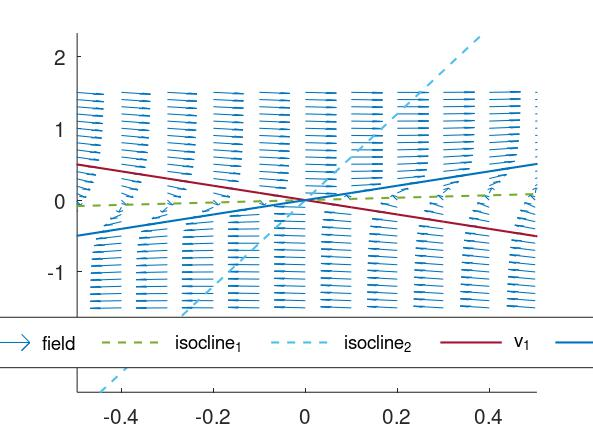
\includegraphics[width=\linewidth]{Phases/P2-015_09.jpg}
  \caption{a = -0.15 et b = 0.9}
  \label{fig:sub2}
\end{subfigure}%
\begin{subfigure}{.5\textwidth}
  \centering
  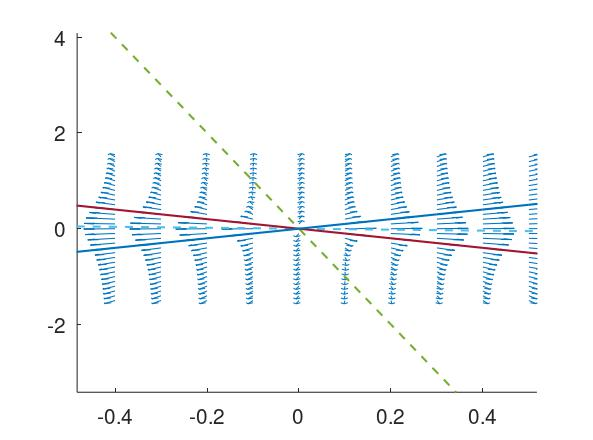
\includegraphics[width=\linewidth]{Phases/P21_01.jpg}
  \caption{a = 1 et b = 0.1}
  \label{fig:sub2}
  \end{subfigure}
\begin{subfigure}{.5\textwidth}
  \centering
  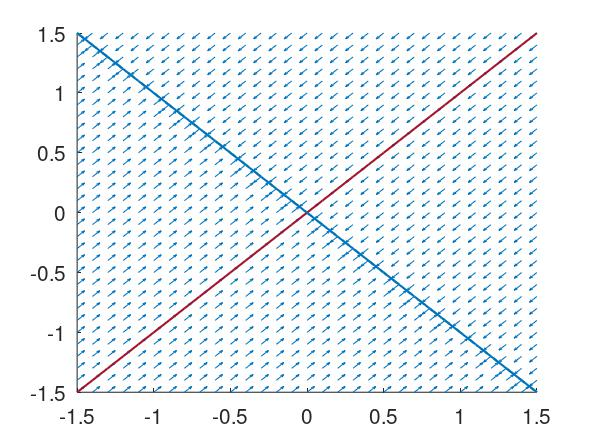
\includegraphics[width=\linewidth]{Phases/P2-01_-01.jpg}
  \caption{a = -0.1 et b = -0.1}
  \label{fig:sub2}
  \end{subfigure}
\begin{subfigure}{.5\textwidth}
  \centering
  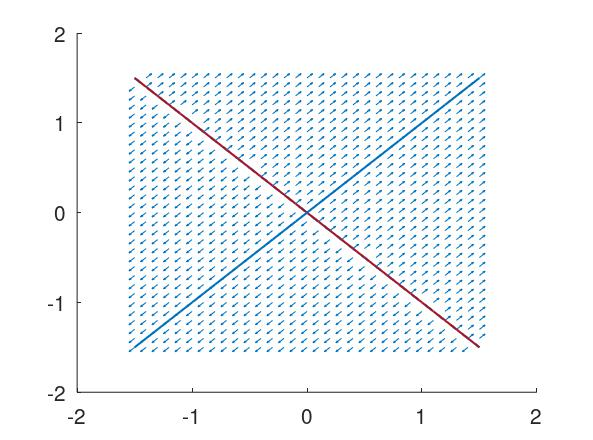
\includegraphics[width=\linewidth]{Phases/P201_01.jpg}
  \caption{a = 0.1 et b = 0.1}
  \label{fig:sub2}
  \end{subfigure}
\caption{Portraits de phase du système 2}
%\label{fig:test}
\end{figure}

\newpage

\subsection{Les deux robots auront une dynamique contrastante}


\begin{equation}
\centering
\left\{\begin{split}
\dot{w}(t) &= aw(t) + be(t)\\
\dot{e}(t) &= - bw(t) - ae(t) \\
\end{split}\right.
 \end{equation}

\begin{equation}
\centering
A = \left[
\begin{array}{cc}
a & b\\
-b & -a
\end{array}
\right]
 \end{equation}

\begin{figure}[!htb]
\centering
\begin{subfigure}{.3\textwidth}
  \centering
  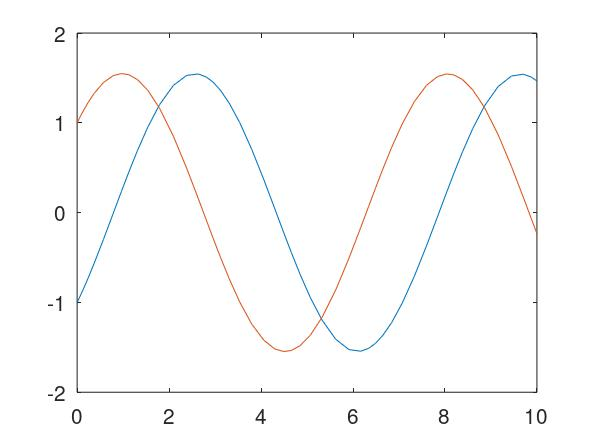
\includegraphics[width=\linewidth]{évol/E3-1_1.jpg}
  \caption{y0 = [-1,1]}
  \label{fig:sub1}
\end{subfigure}%
\begin{subfigure}{.3\textwidth}
  \centering
  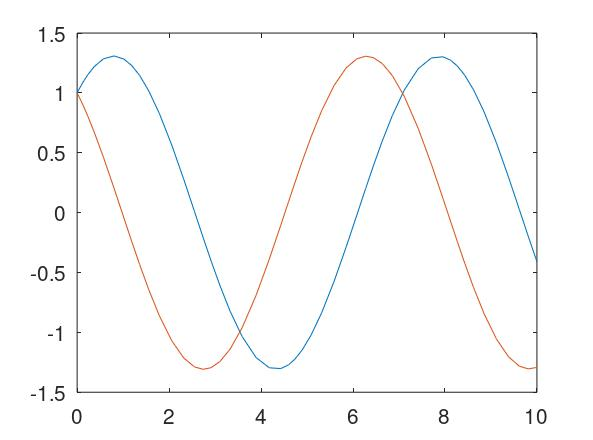
\includegraphics[width=\linewidth]{évol/E31_1.jpg}
  \caption{y0 = [1,1]}
  \label{fig:sub2}
  \end{subfigure}
  \begin{subfigure}{.3\textwidth}
  \centering
  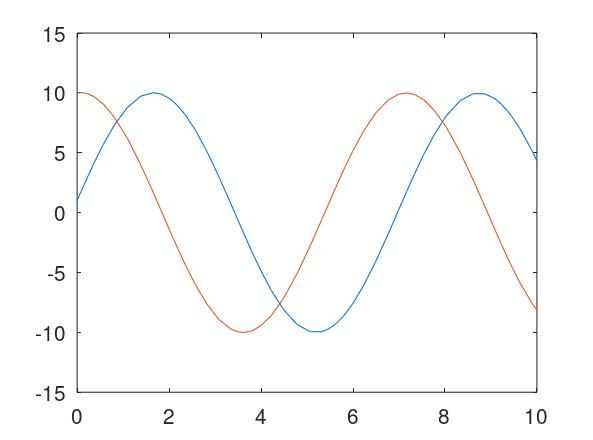
\includegraphics[width=\linewidth]{évol/E31_10.jpg}
  \caption{y0 = [1,10]}
%  \label{fig:sub1}
  \end{subfigure}%
  \begin{subfigure}{.3\textwidth}
  \centering
  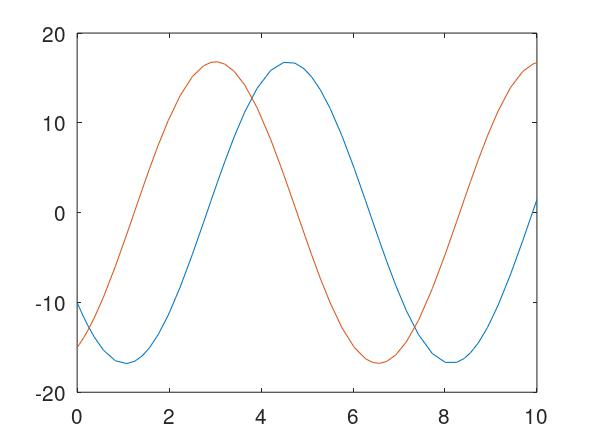
\includegraphics[width=\linewidth]{évol/E3-10_-15.jpg}
  \caption{y0 = [-10,-15]}
%  \label{fig:sub2}
  \end{subfigure}
  \begin{subfigure}{.3\textwidth}
  \centering
  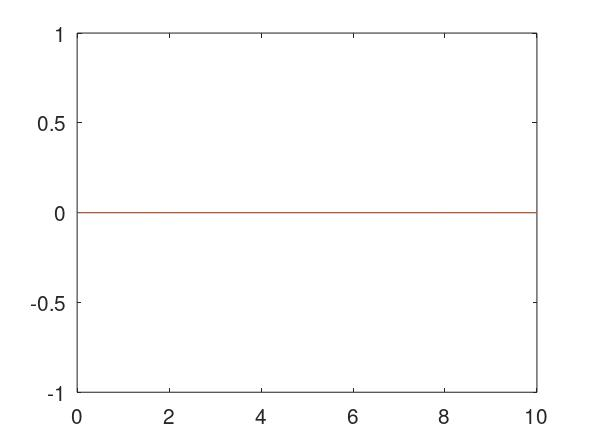
\includegraphics[width=\linewidth]{évol/E20_0.jpg}
  \caption{y0 = [0,0]}
%  \label{fig:sub2}
  \end{subfigure}
\caption{Evolutions du système 3 pour les conditions initiales y0}
%\label{fig:test}
\end{figure}

\subsubsection{Typologie}

Si $(a^2-b^2) < 0$, cela donne un centre. Ici, $(-0.15^2-0.9^2) = -0.7875$
\\
Si $(a^2-b^2) > 0$, cela donne une selle. Ici, $(-1^2-0.1^2) = 0.99$
\\
Si a = b, cela donne un noeud singulier. Ici, a = 0.1 et b = 0.1.
\\

\begin{figure}[!htb]
\centering
\begin{subfigure}{.4\textwidth}
  \centering
  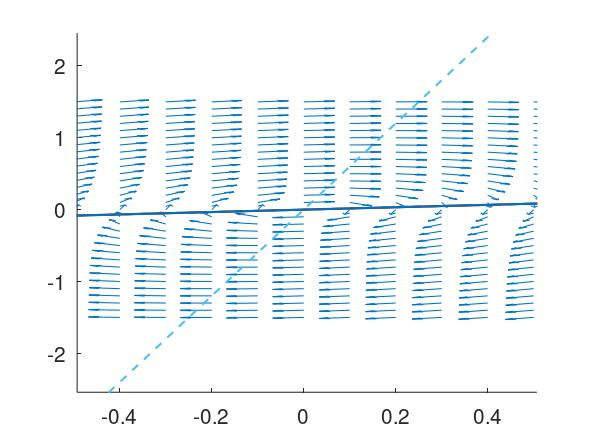
\includegraphics[width=\linewidth]{Phases/P3-015_09.jpg}
  \caption{a = -0.15 et b = 0.9}
  \label{fig:sub1}
\end{subfigure}%
\begin{subfigure}{.4\textwidth}
  \centering
  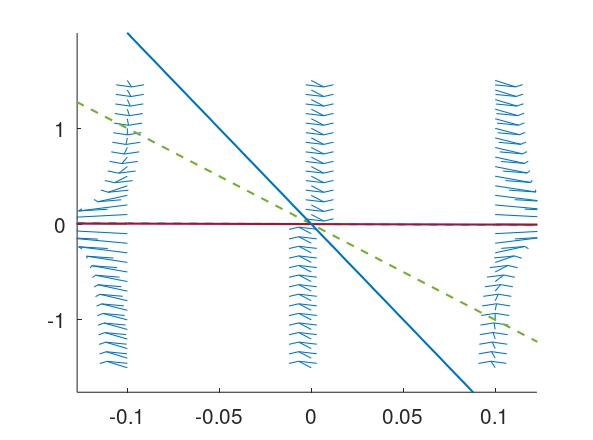
\includegraphics[width=\linewidth]{Phases/P31_01.jpg}
  \caption{a = 1 et b = 0.1}
  \label{fig:sub2}
  \end{subfigure}
\begin{subfigure}{.4\textwidth}
  \centering
  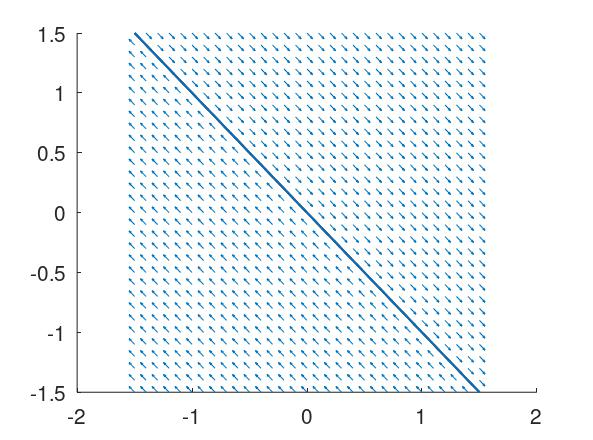
\includegraphics[width=\linewidth]{Phases/P301_01.jpg}
  \caption{a = 0.1 et b = 0.1}
  \label{fig:sub2}
  \end{subfigure}
\caption{Portraits de phase du système 3}
%\label{fig:test}
\end{figure}


\newpage

\subsection{La dynamique de chaque robot dépend simplement de l’autre
robot}

\begin{equation}
\centering
\left\{\begin{split}
\dot{w}(t) &= aw(t) \\
\dot{e}(t) &= bw(t) \\
\end{split}\right.
 \end{equation}

\begin{equation}
\centering
A = \left[
\begin{array}{cc}
a & 0\\
b & 0
\end{array}
\right]
 \end{equation}

\begin{figure}[!htb]
\centering
\begin{subfigure}{.3\textwidth}
  \centering
  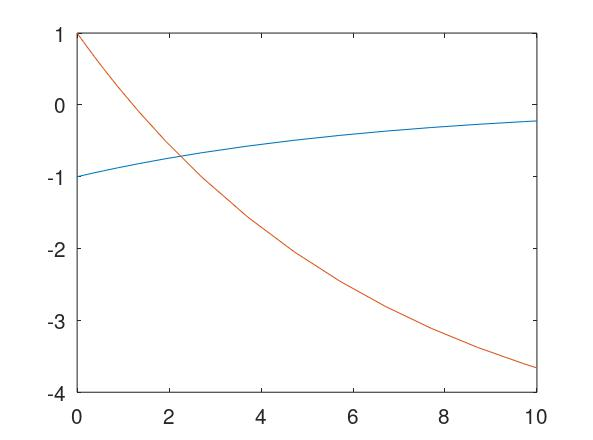
\includegraphics[width=\linewidth]{évol/E4-1_1.jpg}
  \caption{y0 = [-1,1]}
  \label{fig:sub1}
\end{subfigure}%
\begin{subfigure}{.3\textwidth}
  \centering
  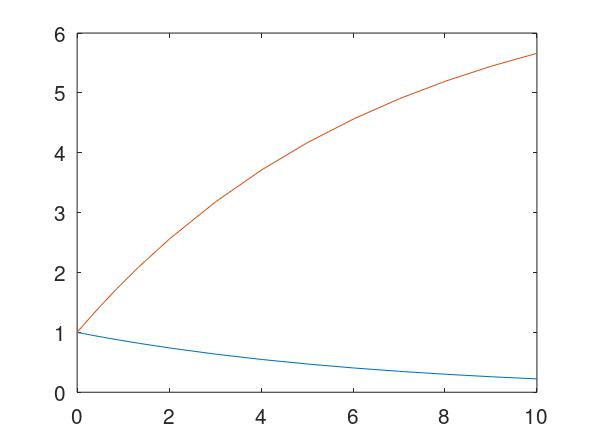
\includegraphics[width=\linewidth]{évol/E41_1.jpg}
  \caption{y0 = [1,1]}
  \label{fig:sub2}
  \end{subfigure}
  \begin{subfigure}{.3\textwidth}
  \centering
  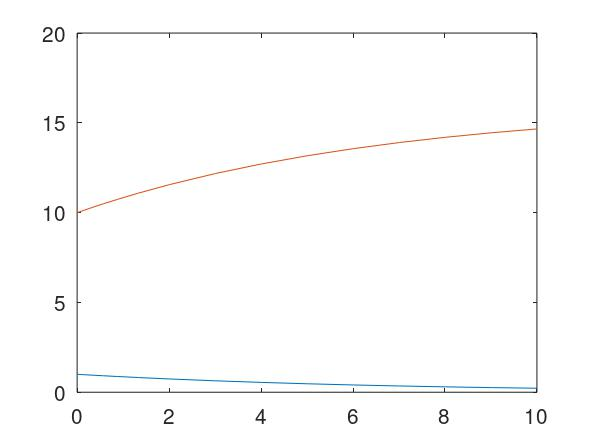
\includegraphics[width=\linewidth]{évol/E41_10.jpg}
  \caption{y0 = [1,10]}
%  \label{fig:sub1}
  \end{subfigure}%
  \begin{subfigure}{.3\textwidth}
  \centering
  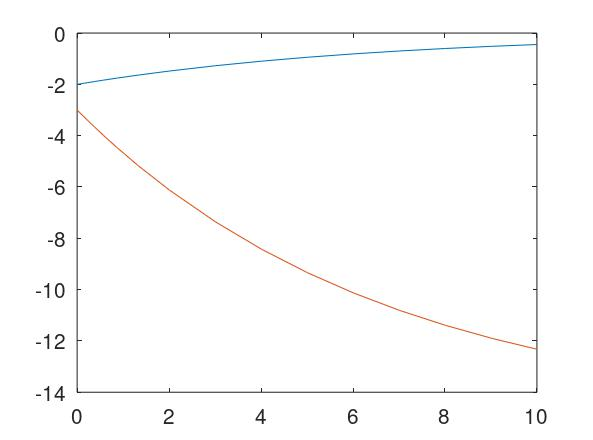
\includegraphics[width=\linewidth]{évol/E4-2_-3.jpg}
  \caption{y0 = [-2,-3]}
%  \label{fig:sub2}
  \end{subfigure}
  \begin{subfigure}{.3\textwidth}
  \centering
  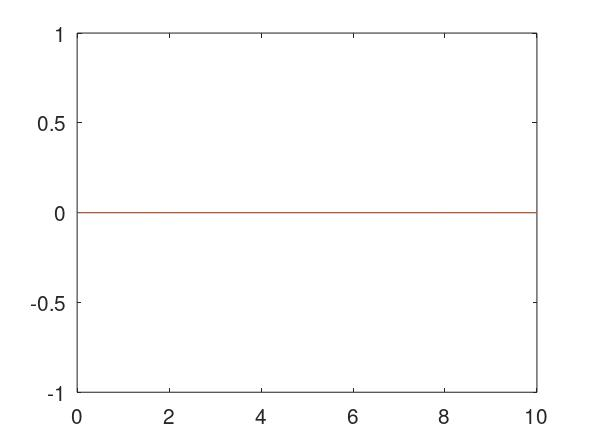
\includegraphics[width=\linewidth]{évol/E20_0.jpg}
  \caption{y0 = [0,0]}
%  \label{fig:sub2}
  \end{subfigure}
\caption{Evolutions du système 4 pour les conditions initiales y0}
%\label{fig:test}
\end{figure}

\subsubsection{Typologie}

Si a $<$ 0, cela donne un noeud stable dégénéré. Ici, a = -0.15 et b = 0.9.
\\
Si a $>$ 0, cela donne un noeud instable dégénéré. Ici, a = -0.15 et b = 0.9.
\\
xxx Si a = 0, cela donne un noeud singulier. Ici a = 0 et b = 1.


\begin{figure}[!htb]
\centering
\begin{subfigure}{.5\textwidth}
  \centering
  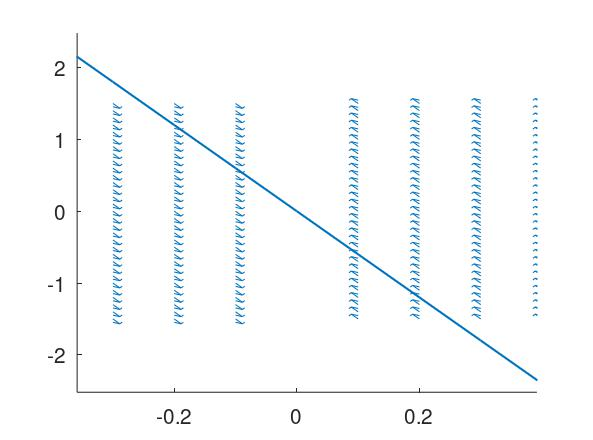
\includegraphics[width=\linewidth]{Phases/P4-015_09.jpg}
  \caption{a = -0.15 et b = 0.9}
  \label{fig:sub1}
\end{subfigure}%
\begin{subfigure}{.5\textwidth}
  \centering
  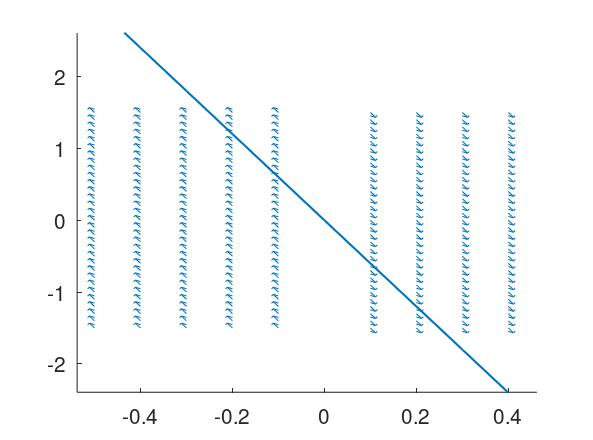
\includegraphics[width=\linewidth]{Phases/P4015_-09.jpg}
  \caption{a = 1 et b = 0.1}
  \label{fig:sub2}
  \end{subfigure}
\caption{Portraits de phase du système 4}
%\label{fig:test}
\end{figure}

\newpage

\subsection{Bonus : a n’est pas une constante mais dépend du temps}

On pose a(t) = max(0, 100 − 0.1t).

\begin{equation}
\centering
\left\{\begin{split}
\dot{w}(t) &= a(t)w(t) + be(t)\\
\dot{e}(t) &= bw(t) + a(t)e(t) \\
\end{split}\right.
 \end{equation}

\end{document}
